\documentclass[conference]{IEEEtran}
\usepackage{graphicx} % Required for inserting images
\usepackage{float}
\usepackage{subcaption}

\def\BibTeX{{\rm B\kern-.05em{\sc i\kern-.025em b}\kern-.08em
    T\kern-.1667em\lower.7ex\hbox{E}\kern-.125emX}}
\begin{document}

\title{Data Mining Project: Analyzing Video Game Sales\\
{\footnotesize \textsuperscript{*} CS 4412: Data Mining}

}

\author{\IEEEauthorblockN{Joshua Vach}
\IEEEauthorblockA{\textit{Student at Kennesaw State University} \\
Marietta GA \\
jvach3@students.kennesaw.edu}

}
\maketitle

\section{Data Preprocessing and Transformation for FPGrowth and Anomaly Detection}
While the data contained in the video game csv database is
mostly full and accurate there are a few missing values mainly
in years which has several games without years labeled as NA
which is simple to deal with pandas dropna command. There
are also several games within the dataset that have 0 sales in
certain sales markets this however is not a problem as they
have data stored there it is just 0.

For the implementation of the FPGrowth algorithm i created 3 indicators indicators where each set is made up of games that performed better than the median sales in each region in order to find what indicators allowed for games to succeed over other games in the same market. Years are also separated into decades in order to create larger groups of games for grouping in FPGrowth.

For the implementation of the Isolation forest anomaly detection algorithm the data was only specified to be the year sales for every region as well as global sales.

\section{FPGrowth Algorithm}
In this deliverable we implemented an FPGrowth algorithm in order to answer our discovery questions. Unlike our implementation of K-means there was no need to create 3 algorithms to answer each question as we created a single implementation that answers all three of our discovery questions. The analysis will be separate for each question but only one figure will be provided at the beginning of the analysis section.

The implementation of FPGrowth takes the input data of 3 datasets of games that performed above the median sales in each region. There are several core attributes that are put into the transactions these include publishers, platform, decade of release, as well as success in Japan, North America, and Europe. The three transactions that will be analyzed are the success in Japan, North America, and Europe.

\begin{figure}[H]
    \centering
    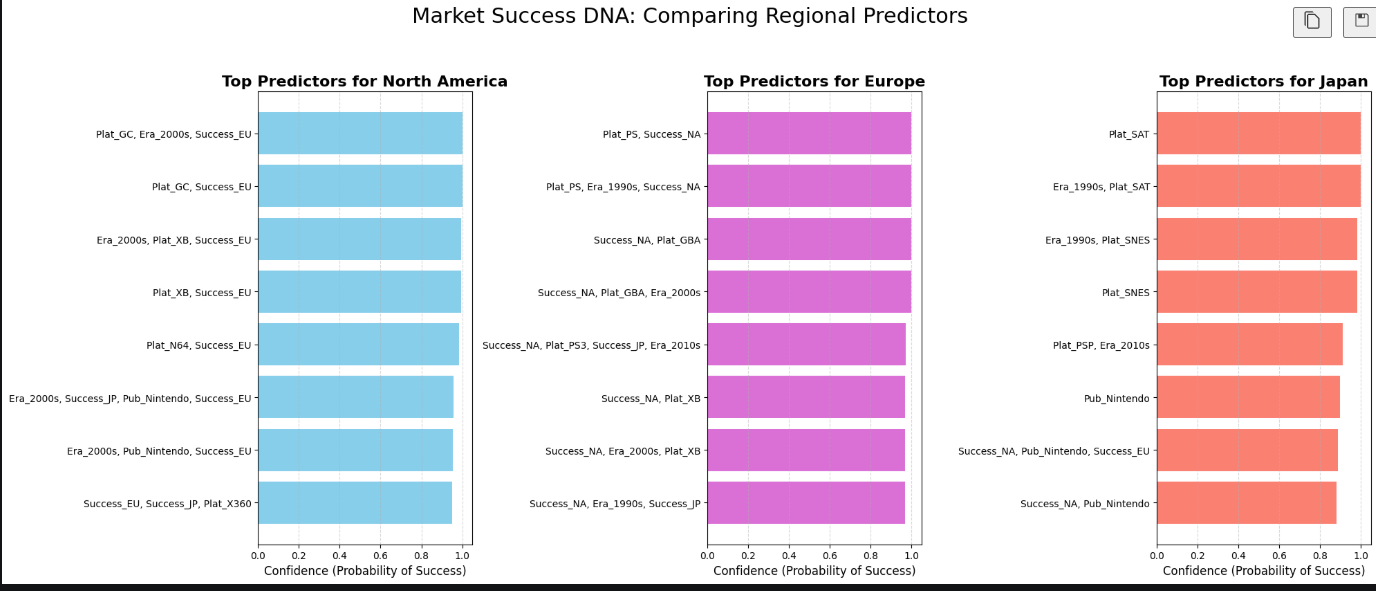
\includegraphics[width=1\linewidth]{DataMiningFPGrowth.png}
    \label{fig:placeholder}
\end{figure}

\subsection{Question 1: Market Success in Home Market Against
Foreign Market}
The success in various markets is shown to have very little to do with the publisher of the game. The platform, decade and success in other markets have much more impact on whether or not a game succeeds in a market. The one exception to this is Nintendo as both in North America and Japan where having Nintendo as the publisher allows for around 90 percent of games sell over the median of sales in that region. While in North America this is tied to the 2000s and success in the EU and Japan, Nintendo publishing with no other indicators in Japan allows for around 90 percent of games to perform better than the median while having the game also succeed in North America actually reduces its success rate in Japan. Since Nintendo is based in Japan it actually does prove that some publishers do perform better in their home market than abroad, but since no other publisher appears on the top indicators it shows that Nintendo is an outlier not the rule especially since it appears so low on the top indicators comparatively to platforms, decades, and success in other markets.

\subsection{Finding Healthy Platform Ecosystems and Successful Platforms}
Indicators for a healthy platform ecosystem in this implementation would be high rates of success for games on a specific platform. There are various platforms shown in the graphs that match this criteria. these include the Game Cube, Xbox, Xbox 360, N64, Playstation, GameBoy Advance, SNES, and surprisingly the Sega Saturn. All of these bar one makes sense as they are some of the most popular consoles of all time meaning they had lots of games and sales. The Xbox seems to be the healthiest across all markets as it is a top indicator for both the North American and European markets. The other platforms only appear in the top 8 indicators in one market. One interesting data point is the Sega Saturn as it failed abroad but was very successful in Japan as releasing on the Saturn as an indicator has 100 percent success rate with games. it is the only platform that does this without another indicator like success in another market. This outlier could be due to the Sega Saturn's marketing inside Japan compared to outside which helped drive more sales and therefore a healthier platform ecosystem inside Japan compared to its ecosystem in other markets.

\subsection{Change in Market share Over Time}
According to indicators of success in the FPGrowth algorithm the 2000s and 1990s have the most successful games as the 2000s appear 5 times in the top 8 of the three markets, and the 1990s appear 4 times. Both these eras are indicators for 100 percent success with both appearing once. The 2010s appear twice showing success is still there but not as much as earlier. This data corroborates the data we found in the k-means as sales began to climb around the 90s and peaked around 2010 before falling by about half and since more success was found in the 1990s and 2000s, 4 and 5 respectively, than the 2010s, only 2 appearances, the data found in the FPGrowth tracks the trend we found previously.

\section{Anomaly Detection}
For our Anomaly Detection algorithm we implemented the Isolation Forest algorithm. The data points we are using to determine anomalies are the year, sales in different regions, and global sales. This is to determine if there are any anomalies with sales in different regions.

\begin{figure}[H]
    \centering
    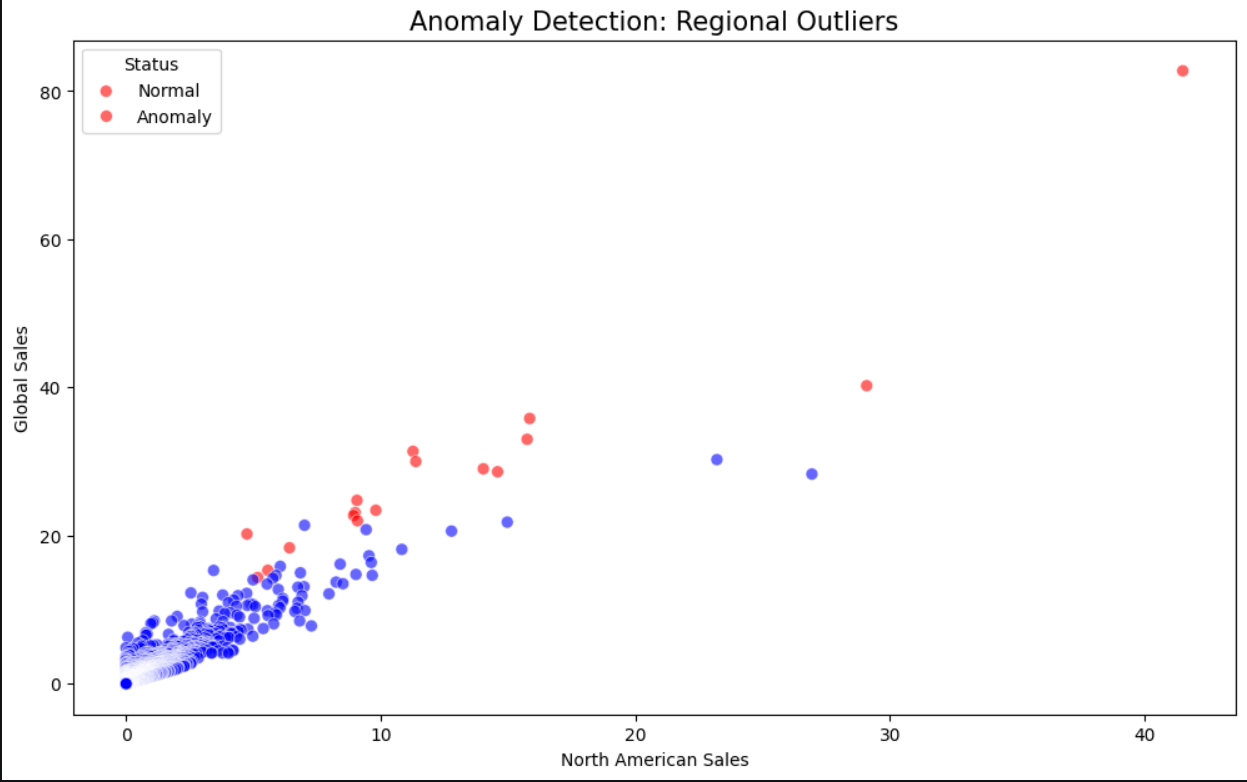
\includegraphics[width=1\linewidth]{DataMiningNAAnomaly.png}
    \label{fig:placeholder}
\end{figure}
\begin{figure}[H]
    \centering
    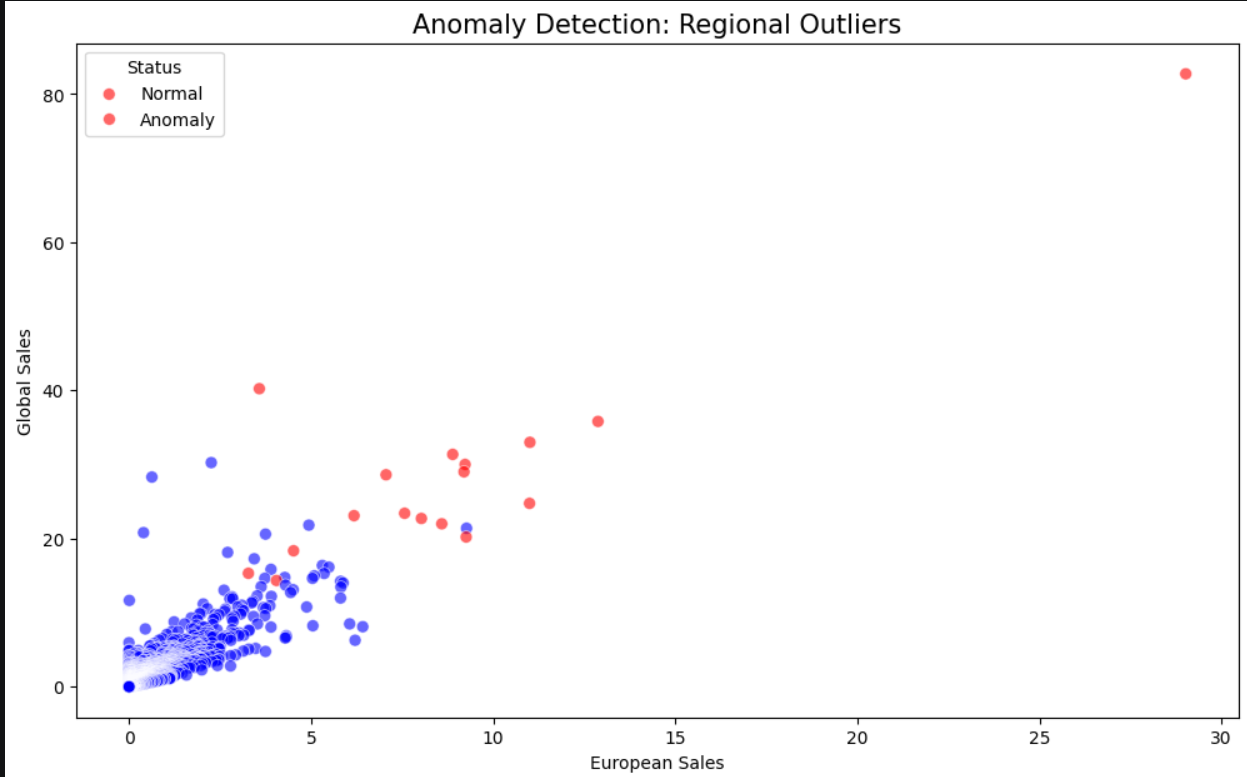
\includegraphics[width=1\linewidth]{DataMiningEUAnomaly.png}
    \label{fig:placeholder}
\end{figure}
\begin{figure}[H]
    \centering
    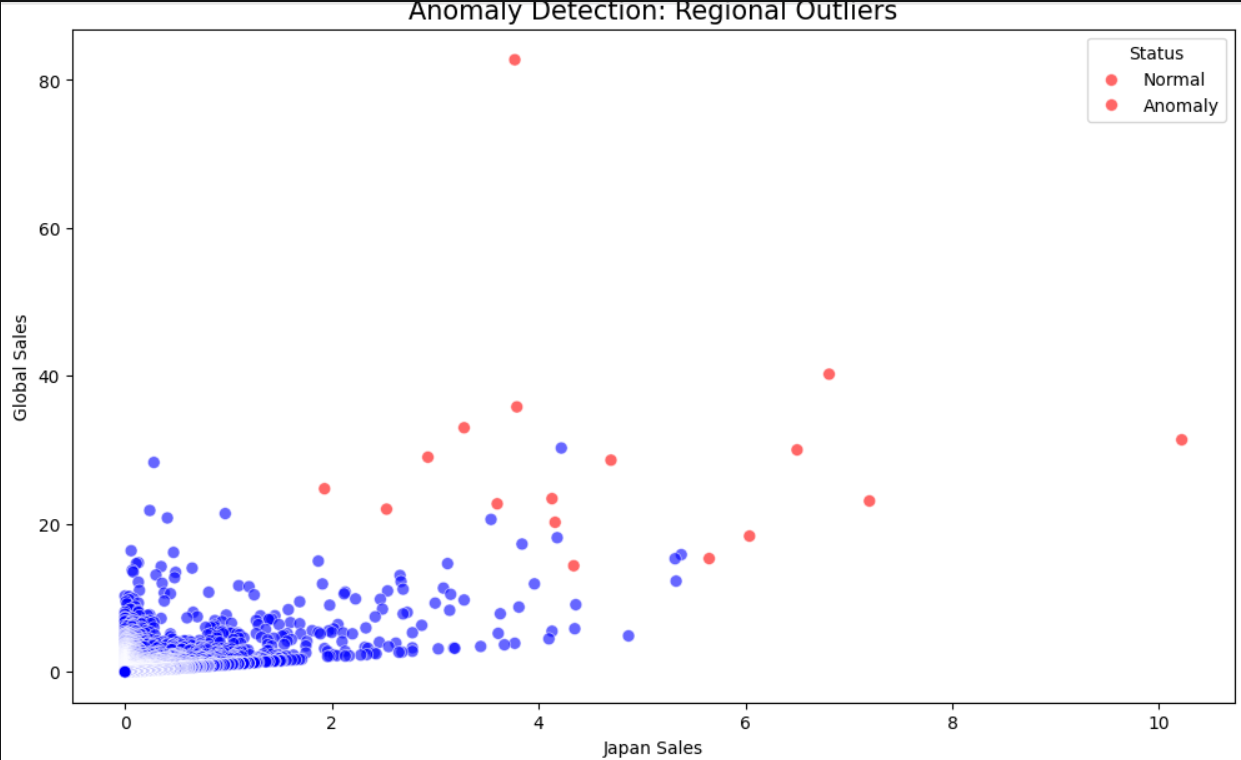
\includegraphics[width=1\linewidth]{DataMiningJPAnomaly.png}
    \label{fig:placeholder}
\end{figure}

The top 10 anomalous data points are all in the top 20 best selling games and all are published by Nintendo. Six of them are Wii games and three are DS games with one being a GameBoy game. All are incredibly well known games like Mario, Wii Sports, or Pokemon with the exception of one that being "Brain Age: Train Your Brain in Minutes a Day" which is the 20th best selling game of all time with most of it coming from Europe which would explain it being flagged as Anomalous. This shows that Nintendo is one of the few publishers that can perform well regardless of market as the anomalous data points are  mostly Nintendo showing they can over perform in markets they typically shouldn't do well in. This shows that while the findings in the FPGrowth show Nintendo performs well in its home region this is less of a symptom of publishers as a whole, but the fact that Nintendo is most likely an outlier among publishers.

\section{M4 Plan}
All of the implementations are functional and provide accurate results there are a few things that need to be worked on to clean up results. One thing would be to print out the stats for all anomalies as there are so few of them that it can easily be printed alongside making the graphs look more professional. The third K-means algorithm's graph also could use some changes as there is an outlier currently printed onto the graph. The FPGrowth graph could also be expanded to show more indicators for a better showcase of various trends.
\end{document}
